\documentclass[aspectratio=169,10pt]{beamer}
\usetheme{default}
\usecolortheme{dolphin}
\usepackage{amsmath,amssymb,booktabs,tikz,pgfplots}
\usetikzlibrary{arrows.meta,positioning,calc}
\pgfplotsset{compat=1.17}
\setbeamertemplate{navigation symbols}{}
\setbeamertemplate{footline}{\hfill\insertframenumber/\inserttotalframenumber\hspace{1em}\vspace{0.6em}}
\definecolor{hblue}{RGB}{25,91,164}
\definecolor{eorange}{RGB}{210,105,30}
\setbeamercolor{structure}{fg=hblue}
\title{How Large Is the Hyperbolic Advantage?}
\subtitle{A strong-baseline audit for multimodal retrieval}
\author{Teng Long}
\date{October 2026}

\begin{document}
\begin{frame}
  \titlepage
  \vspace{-1.2em}
  \centering\small Reproducible deck: frozen recipes, five seeds, rank-based evidence
\end{frame}

\begin{frame}{Take-away: useful on one regime, not universal}
\begin{columns}[T]
\column{0.49\linewidth}
\begin{block}{What survives the audit}
\begin{itemize}
\item Direct Lorentz lift + full-training LoRA is the strongest H variant.
\item Development: a local sweet spot at 128-D.
\item Full-corpus NanoSciFact improves at both 128-D and 256-D.
\end{itemize}
\end{block}
\column{0.49\linewidth}
\begin{alertblock}{What does not survive}
\begin{itemize}
\item No broad win on the 97-task MMEB-v3 screen.
\item Video/image retrieval does not reliably improve.
\item Raw cosine/E/H margins are not on a shared absolute scale.
\end{itemize}
\end{alertblock}
\end{columns}
\vfill
\centering\large The result is \textbf{task-conditional evidence}, not a universal geometry claim.
\end{frame}

\begin{frame}{Why hyperbolic space suggests larger capacity}
For the unit-curvature Lorentz model,
\[
\mathbb H^n=\{x:\langle x,x\rangle_L=-1,\ x_0>0\},\qquad
ds^2=dR^2+\sinh^2R\,d\Omega_{n-1}^2.
\]
Thus shell area grows as $\sinh^{n-1}R=\Theta(e^{(n-1)R})$.

For two equal-radius points separated by angle $\theta$,
\[
\cosh d_H=1+\sinh^2R(1-\cos\theta),\qquad
d_H\approx 2R+2\log\theta-\log4.
\]
If $N$ directions require $\theta\asymp N^{-1/(n-1)}$, constant separation needs
$R_H=O(\log N)$, versus polynomial Euclidean radius.

\begin{alertblock}{Scope}
This is a representational-capacity argument under a shell-packing model. It does not
guarantee that optimization, data, or downstream ranking realizes the capacity.
\end{alertblock}
\end{frame}

\begin{frame}{Final method: H10 is a hybrid Lorentz retriever}
\centering
\resizebox{0.96\textwidth}{!}{%
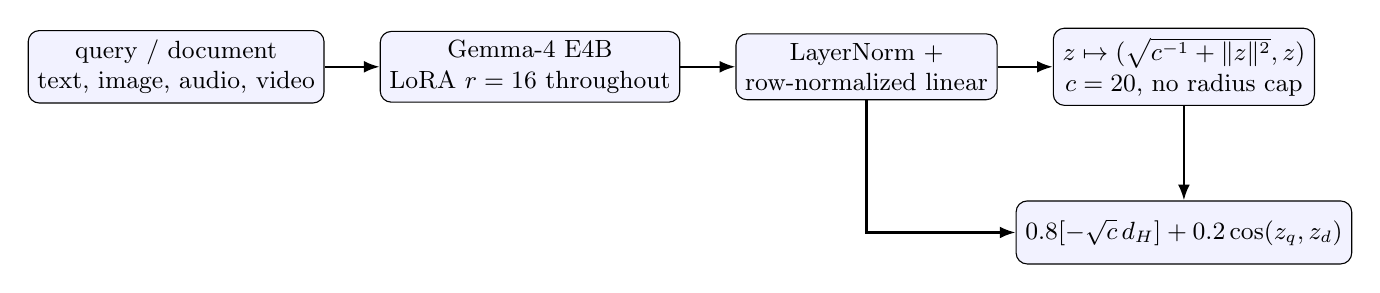
\begin{tikzpicture}[node distance=7mm and 7mm, every node/.style={font=\small},
box/.style={draw,rounded corners,minimum height=8mm,align=center,fill=blue!5},
arr/.style={-{Latex[length=2mm]},thick}]
\node[box] (input) {query / document\\text, image, audio, video};
\node[box,right=of input] (gemma) {Gemma-4 E4B\\LoRA $r=16$ throughout};
\node[box,right=of gemma] (head) {LayerNorm +\\row-normalized linear};
\node[box,right=of head] (lift) {$z\mapsto(\sqrt{c^{-1}+\|z\|^2},z)$\\$c=20$, no radius cap};
\draw[arr] (input)--(gemma); \draw[arr] (gemma)--(head); \draw[arr] (head)--(lift);
\node[box,below=12mm of lift] (score) {$0.8[-\sqrt c\,d_H]+0.2\cos(z_q,z_d)$};
\draw[arr] (lift)--(score); \draw[arr] (head.south) |- (score.west);
\end{tikzpicture}
}

\vspace{1em}
Symmetric hard-negative InfoNCE; 7 online negatives; batch $8\times2$ accumulation;
256 steps; no explicit margin loss. Cosine is computed \emph{before} the lift.
\end{frame}

\begin{frame}{A fair comparison requires a strong Euclidean baseline}
\begin{columns}[T]
\column{0.49\linewidth}
\textbf{Independent tuning}
\begin{itemize}
\item 38 recipes $\times$ 3 seeds per geometry
\item top 8 recipes $\times$ 2 new seeds
\item same backbone, LoRA rank, training data, hard-negative count
\end{itemize}
\column{0.49\linewidth}
\textbf{Matched-step Euclidean arm}
\begin{itemize}
\item 256 steps / 16 warmup
\item $R_{\max}=2$, $\tau=0.14$
\item 0.2 pre-lift cosine mixture
\item independent best head LR $2.5\times10^{-4}$
\end{itemize}
\end{columns}
\begin{block}{Interpretation rule}
Systems differ in selected hyperparameters beyond geometry. This is a selected-system
comparison, not a curvature-only causal intervention.
\end{block}
\end{frame}

\begin{frame}{Development ablation: a local 128-D advantage}
\centering
\begin{tikzpicture}
\begin{axis}[width=0.88\linewidth,height=0.48\textheight,
xlabel={embedding dimension},ylabel={development macro MRR},
xmode=log,log basis x=2,xtick={32,64,128,256},
ymin=0.72,ymax=0.86,grid=major,legend pos=south east]
\addplot+[orange!85!black,mark=square*,thick,error bars/.cd,y dir=both,y explicit] coordinates {(32,0.751543) +- (0,0.019708) (64,0.766191) +- (0,0.015587) (128,0.779694) +- (0,0.011786) (256,0.796260) +- (0,0.019372)};
\addlegendentry{Euclidean}
\addplot+[blue,mark=*,thick,error bars/.cd,y dir=both,y explicit] coordinates {(32,0.770084) +- (0,0.026747) (64,0.793553) +- (0,0.024392) (128,0.819962) +- (0,0.023271) (256,0.814508) +- (0,0.021450)};
\addlegendentry{Lorentz}
\end{axis}
\end{tikzpicture}

\vspace{-0.8em}
\small Five matched seeds on CIRR, ChartQA, WebQA. At 128-D: $H-E=+0.0403$
[95\% CI $+0.0111,+0.0694$], wins 5/5. At 256, 64, and 32-D the CI crosses zero.
\end{frame}

\begin{frame}{Frozen MMEB-v3 full-corpus confirmation}
\begin{columns}[c]
\column{0.56\linewidth}
\centering\begin{tikzpicture}
\begin{axis}[width=0.92\linewidth,height=0.42\textheight,
xlabel={H $-$ E on official task metric},symbolic y coords={Nano,MS-COCO,MSR-VTT,Clotho},
ytick=data,xmin=-0.04,xmax=0.105,grid=major,axis y line*=left]
\addplot+[only marks,blue,mark=*,mark size=2.4pt,
error bars/.cd,x dir=both,x explicit] coordinates {(0.058952,Nano) += (0.029273,0) -= (0.029272,0) (-0.004545,MS-COCO) += (0.014796,0) -= (0.014797,0) (-0.010000,MSR-VTT) += (0.019747,0) -= (0.019747,0) (0.000191,Clotho) += (0.000994,0) -= (0.000994,0)};
\draw[dashed,gray] (axis cs:0,Nano) -- (axis cs:0,Clotho);
\end{axis}
\end{tikzpicture}

\column{0.42\linewidth}
\centering\scriptsize\begin{tabular}{@{}lrrr@{}}
\toprule
Task & $E$ & $H$ & $H-E$ \\
\midrule
NanoSciFact & 0.2258 & 0.2847 & +0.0590 \\
MS-COCO T$	o$I & 0.0982 & 0.0936 & -0.0045 \\
MSR-VTT & 0.0682 & 0.0582 & -0.0100 \\
Clotho & 0.0006 & 0.0008 & +0.0002 \\
\bottomrule
\end{tabular}

\vspace{0.8em}

\raggedright\small At 128-D, only NanoSciFact is positive with a non-crossing CI:
$+0.0590$ nDCG@5, five wins in five seeds. Removing NanoSciFact, the other three-task
macro delta is $-0.0048$ and crosses zero.
\end{columns}
\end{frame}

\begin{frame}{The broad screen is the necessary negative result}
\centering\small
\begin{tabular}{@{}rrrrrr@{}}
\toprule
Dim & $E$ & $H$ & $H-E$ [95\% CI] & W/T/L \\
\midrule
128 & 0.2487 & 0.2447 & -0.0040 [-0.0188, +0.0108] & 40/2/55 \\
256 & 0.2626 & 0.2596 & -0.0030 [-0.0192, +0.0133] & 41/3/53 \\
\bottomrule
\end{tabular}


\vspace{1em}
\begin{columns}[T]
\column{0.49\linewidth}
\textbf{128-D ranking transitions}
\begin{itemize}
\item relevant rank: 11,183 improved / 5,524 tied / 12,228 worsened
\item top-1: 1,558 became correct / 1,547 became wrong
\end{itemize}
\column{0.49\linewidth}
\textbf{Hard negatives}
\begin{itemize}
\item 21,030 demoted / 691 promoted / 7,214 tied
\item demotion alone does not imply better official metrics
\end{itemize}
\end{columns}
\vfill
\scriptsize Bounded pool: at most 64 queries and 1,024 candidates, with qrels used only
to retain positives. This is a diagnostic screen, not an official full-corpus score.
\end{frame}

\begin{frame}{Where does it work? Current best hypothesis}
\begin{columns}[T]
\column{0.48\linewidth}
\begin{block}{Supports H10}
\begin{itemize}
\item NanoSciFact: text retrieval with scientific topical structure
\item bounded MultiConIR People / Movies: positive at both dimensions (uncorrected)
\item 128-D development sweet spot
\end{itemize}
\end{block}
\column{0.48\linewidth}
\begin{alertblock}{Does not support H10}
\begin{itemize}
\item MS-COCO text-to-image
\item MSR-VTT video retrieval
\item Clotho audio retrieval
\item VisDoc family at 128-D
\end{itemize}
\end{alertblock}
\end{columns}
\vspace{0.8em}
\centering The emerging signal is \textbf{semantic/hierarchical text structure}, not
omni-modality by itself. This hypothesis requires a new pre-registered test.
\end{frame}

\begin{frame}{Related work and what is different here}
\small
\begin{tabular}{@{}p{0.24\linewidth}p{0.31\linewidth}p{0.37\linewidth}@{}}
\toprule
Line & Representative work & Difference in this audit \\
\midrule
Multimodal embedding & CLIP; VLM2Vec; GME; MM-Embed & Strong MLLM embeddings and broad benchmarks, usually Euclidean/cosine \\
Hyperbolic representation & Poincar\'e embeddings; Lorentz embeddings & Hierarchy capacity and stable Lorentz optimization \\
Hyperbolic vision-language & MERU; HyCoCLIP; PHyCLIP; HALO & Direct lift and entailment/compositional objectives \\
This work & Gemma-4 + MMEB-v3 & Independently tuned E/H systems, dimension ablation, broad negative result, frozen full-corpus confirmation \\
\bottomrule
\end{tabular}
\vspace{1em}
\scriptsize Key references: Nickel \& Kiela (NeurIPS 2017; ICML 2018); Desai et al.
(ICML 2023); Pal et al. (ICLR 2025); Huang et al. (MMEB-v3, 2026); Ratcliffe
(\emph{Foundations of Hyperbolic Manifolds}, 2019).
\end{frame}

\begin{frame}{Conclusions and next falsifiable experiment}
\begin{enumerate}
\item Hyperbolic volume growth gives a clean \emph{capacity mechanism}, not an automatic ranking win.
\item H10 beats the matched Euclidean system at 128-D on development and on full-corpus NanoSciFact.
\item It does not improve the 97-task screen overall; multimodal transfer remains weak.
\item Cross-geometry raw distance margins are not evidence; rankings and official metrics are.
\end{enumerate}
\begin{block}{Next test}
Pre-register a text-heavy hierarchy suite, tune neither geometry on its qrels, and compare
32/64/128/256-D with at least five new seeds. The hypothesis is that H helps when candidate
structure is genuinely hierarchical, especially under moderate compression.
\end{block}
\vfill
\centering\small All numbers and figures in this deck regenerate with \texttt{make reproduce}.
\end{frame}
\end{document}
